\documentclass{IEEEtran}
\usepackage{cite}
\usepackage{amsmath}
\usepackage{graphicx}
\usepackage{booktabs}
\usepackage{lipsum}
\usepackage{authblk}
\graphicspath{{images/}}

\title{A Review on Neural Language Modeling}
\author{Anuar Maratkhan}
\affil{School of Science and Technology\\Nazarbayev University\\anuar.maratkhan@nu.edu.kz}
\renewcommand\Authands{ and }
\begin{document}
\maketitle

\begin{abstract}
Language modeling (LM) appears to be a main task of natural language processing (NLP). Language modeling is also known as statistical language modeling due to large number of statistical approaches. However, in the last decade neural language models became more popular due to higher performance results. The study will therefore, review some of the previous and current state-of-the-art neural language models, and present different studies involved word-level, subword-level recurrent neural network approaches, even those trained with reinforcement learning method. The study then ends by summing up those discussions and giving some future work suggestions.
\end{abstract}

\section{Introduction}

Language Modeling (LM) is a central task in Natural Language Processing (NLP) and play main role in speech recognition, machine translation, optical character recognition, natural language understanding, question answering and many other tasks. Language modeling is all about sequential data. \textit{Language model} is an algorithm for predicting next word in a text given preceeding ones (figure \ref{fig:sequence}). It is also mostly known as \textit{statistical language model} for its richness in statistical approaches in previous works. The state-of-the-art statistical language models turned up to be cache models and class-based models. In addition, according to \cite{Mikolov2010NeuralLM}, most of the statistical models require more data for better performance. 

\begin{figure}[h]
	\centering
	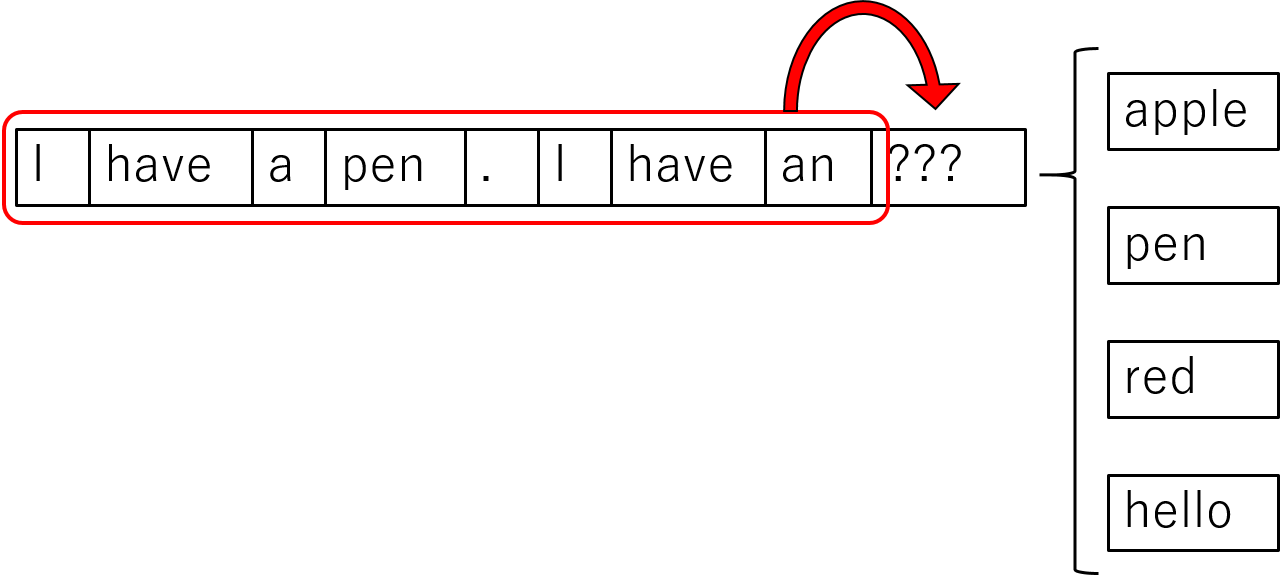
\includegraphics[width=0.45\textwidth]{sequence}
	\caption{Next word prediction in a text.}
	\label{fig:sequence}
\end{figure}

However, as soon as neural networks became popular, \textit{neural language modeling} approaches were invented. Artificial neural networks perform well on supervised learning tasks (when the data is \textit{labeled}) and unsupervised learning tasks (when the data is \textit{unlabeled}). Quoc V. Le et al. in their study \cite{unsupervised} explored and demonstrated how well neural networks operate on unsupervised learning task, where a model has to detect whether a given image contains a face or not. And as the study \cite{unsupervised} notes, the work has been motivated by neuroscience hypothesis. So does the whole science about neural networks. Moreover, information retrieval tasks that are mainly composed of unlabeled data, like in search engines, can be approached by such unsupervised learning techniques. Neural language models, also known as continous-space language models, make use of these neural networks. Those are current state-of-the-art approaches in language modeling.

In the second section of this paper we start by defining what the Recurrent Neural Network (RNN) is, and how it can be applied to language modeling. Studies \cite{Mikolov2010NeuralLM}, \cite{Mikolov2011ExtensionsOR}, \cite{Zaremba2014LSTM}, \cite{Salakhutdinov2017Softmax} show that RNNs seem to be best techniques for language modeling in terms of performance. Thus, RNN appears to be a main approach for neural language modeling nowadays but not the only one. Hence, we proceed by reviewing other interesting approaches to neural language modeling such like subword-level language models presented in \cite{Mikolov2011SubwordLM} and reinforcement learning based language models like in \cite{Quoc2017Reinforcement}. We continue by concluding the review of artificial neural science applied in language modeling. At the end, we present our future suggestions on the neural language modeling approaches. 

\section{Recurrent Neural Networks based Language Models}

\subsection{Recurrent Neural Network}

Recurrent Neural Networks (RNN) are primarily used in sequential data analysis such as video processing, text processing, predicting stock prices and other. RNN architecture is an improvement of feed-forward networks that takes into account previous hidden layer results by storing them in memory. An invention of backpropogation caused an exciting use of RNNs \cite{deeplearning}.

Simple recurrent neural network used in \cite{Mikolov2010NeuralLM} can be described by input at time \(t\) -- \(x(t)\), hidden layer at time \(t\) -- \(s(t)\), and the output layer at time \(t\) -- \(y(t)\), which are computed as follows:

\begin{equation}
	x(t) = w(t) + s(t-1)
\end{equation}
\begin{equation}
	s_j(t) = f\Bigg(\sum_i{x_i(t)u_ji}\Bigg)
\end{equation}
\begin{equation}
	y_k(t) = g\Bigg(\sum_j{s_j(t) v_kj}\Bigg)
\end{equation}

where (1) uses current word at time \(t\) and previous hidden layer at time \(t-1\) as input, (2) and (3) have weights \(u\) and \(v\) used for computations, and both also have sigmoid activation function and softmax function, which are:

\begin{equation}
	f(z) = \frac{1}{1+e^{-z}}
\end{equation}
and
\begin{equation}
	g(z_m) = \frac{e^{z_m}}{\sum_k{e^{z_k}}}
\end{equation}
respectively.

The problem of simple RNN is that the backpropogated gradients vanish or explode \cite{rnn}. That means that simple recurrent neural network model can not store long context but just several preceeding words. Therefore, the improvement in RNN architecture further was introduced with invention of Long-Short Term Memory (LSTM). The LSTM solved the vanishing gradient problem by having special cells with activation gates that provided the model to store longer context. Moreover, Gated Recurrent Unit (GRU) improved the architecture of the LSTM by combining two gates that made the model simpler. The study \cite{rnn} shows that RNNs perform better than complex statistical approaches, N-grams, on a real-world data.

\subsection{Language Models}

Neural language models have demonstrated relatively superior performance on language modeling and speech recognition tasks in comparison to the state-of-the-art statistical approaches, class-based models, in the last decades. Neural language models take their first steps from taking the advantage of feed-forward networks that are listed in \cite{Mikolov2010NeuralLM}, which motivated T. Mikolov et al. to investigate the performance of more advanced type of neural network, RNN. The study was first to evaluate RNN for modeling such sequential data.

In contrast to feed-forward networks that use fixed size of context to predict next word in a sequence, RNNs does not require to use limited number of preceeding words \cite{Mikolov2010NeuralLM}. In other words, RNNs have dynamic size of context in memory. The basic structure of simple recurrent neural network used in the study is shown in figure \ref{fig:rnn} below.

\begin{figure}[h]
	\centering
	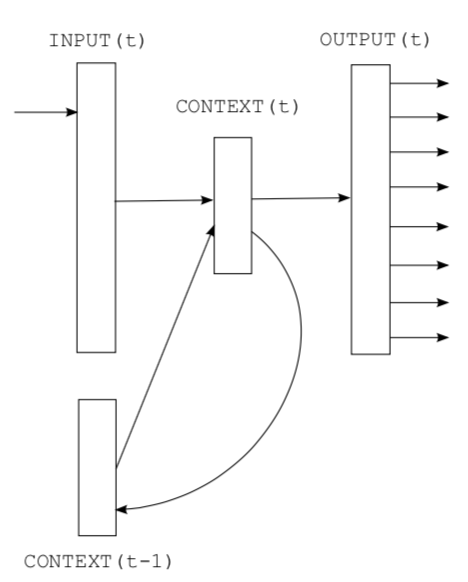
\includegraphics[width=0.3\textwidth]{rnn}
	\caption{Simple recurrent neural network from \cite{Mikolov2010NeuralLM}}
	\label{fig:rnn}
\end{figure}

According to \cite{Mikolov2010NeuralLM} results RNNs illustrated excellent performance relative to best backoff models even being trained on less data than the second ones. The performance in language modeling is measured by \textit{perplexity} which illustrates how well the model can predict next words in a sequence. The lower the perplexity is, the higher the performance. On the other hand, the higher the perplexity, the lower the performance of a particular language model.

Furthermore, \cite{Mikolov2011ExtensionsOR} work presents that RNN based LM can achieve higher efficiency on language modeling tasks by being trained with backpropogation through time (BPTT) optimization technique, which serves as an extension to standard backpropogation algorithm. This backpropogation algorithm is main optimization technique of neural network models. The backpropogation is basically updating neural network weights (coefficients) iteratively. The key concept of BPTT is that the error propogates back for several time steps through its recurrent connections, as it was stated in \cite{Mikolov2011ExtensionsOR}.

Later, Zaremba et al. were first to implement LSTM model with dropout regularization for language modeling task, and demonstrated another improvements in perplexity \cite{Zaremba2014LSTM}. Moreover, subsequent studies listed in \cite{Salakhutdinov2017Softmax} show other improvements in perplexity with LSTMs and other techniques on word-level language modeling. Short overview on the work done there illustrated in table \ref{tab:softmax}\footnote{It is out of scope of this paper to provide detailed description of those approaches.}.

In general, recurrent networks are expected to improve natural language understanding in real-world applications. These also involves language modeling tasks.

% Table 1
\begin{table*}[!t]
\caption{Single model perplexity on validation and test sets on Penn Treebank \cite{Salakhutdinov2017Softmax}.}
\label{tab:softmax}
\centering
\begin{tabular}{ l|c c c }
\toprule
\textbf{Model} & \textbf{#Param} & \textbf{Validation} & \textbf{Test} \\
\hline
Mikolov \& Zweig (2012) -- RNN-LDA + KN-5 + cache & 9M & - & 92.0 \\
Zaremba et al. (2014) -- LSTM & 20M & 86.2 & 82.7 \\
Gal \& Ghahramani (2016) -- Variational LSTM (MC) & 20M & - & 78.6 \\
Kim et al. (2016) -- CharCNN & 19M & - & 78.9 \\
Merity et al. (2016) -- Pointer Sentinel-LSTM & 21M & 75.7 & 70.9 \\
Grave et al. (2016) -- LSTM + continuous cache pointer & - & - & 72.1 \\
Inan et al. (2016) -- Tied Variational LSTM + augmenter loss & 24M & 75.7 & 73.2 \\
Zilly et al. (2016) -- Variational RHN & 23M & 67.9 & 65.4 \\
Zoph \& Le (2016) -- NAS Cell & 25M & - & 64.0 \\
Melis et al. (2017) -- 2-layer skip connection LSTM & 24M & 60.9 & 58.3 \\
\hline
Merity et al. (2017) -- AWD-LSTM w/o finetune & 24M & 60.7 & 58.8 \\
Merity et al. (2017) -- AWD-LSTM & 24M & 60.0 & 57.3 \\
Salakhutdinov et al. \cite{Salakhutdinov2017Softmax} -- AWD-LSTM-MoS w/o finetune & 22M & 58.08 & 55.97 \\
Salakhutdinov et al. \cite{Salakhutdinov2017Softmax} -- AWD-LSTM-MoS & 22M & \textbf{56.54} & \textbf{54.4} \\
\hline
Merity et al. (2017) -- AWD-LSTM + continous cache pointer & 24M & 53.9 & 52.8 \\
Krause et al. (2017) -- AWD-LSTM + dynamic evaluation & 24M & 51.6 & 51.1 \\
Salakhutdinov et al. \cite{Salakhutdinov2017Softmax} -- AWD-LSTM-MoS + dynamic evaluation & 22M & \textbf{48.33} & \textbf{47.69} \\
\bottomrule
\end{tabular}
\end{table*}

% Table 2
\begin{table*}[!t]
\caption{Single model perplexity on the test set of the Penn Treebank language modeling task \cite{Quoc2017Reinforcement}.}
\label{tab:search}
\centering
\begin{tabular}{ l|c c }
\toprule
\textbf{Model} & \textbf{Parameters} & \textbf{Test Perplexity} \\
\hline
Neural Architecture Search with base 8 & 32M & 67.9 \\
Neural Architecture Search with base 8 and shared embeddings & 25M & 64.0 \\
Neural Architecture Search with base 8 and shared embeddings & 54M & 62.4 \\
\bottomrule
\end{tabular}
\end{table*}

\section{Other Language Models}
\subsection{Subword-level Language Modeling}

All of the studies discussed before involved word-level language modeling approaches. Word-level language models have particular size of vocabulary that indicates number of \textit{unique} words learned in the process of training. Even though those models show relatively superior performance in terms of lower perplexity and number of parameters, when it comes to new words (during evaluation on the test set) that have not appeared throughout training, the word-level language models are unable to assign nonzero probability of occurence to those unknown Out-of-Vocabulary (OOV) words. As a consequence, the models incapable to use OOV words to predict next word in the sequence. If the OOV words are rare words that occur in the texts not so often, it is not that dangerous. But when the OOV words are not rare and occur often, OOV words become a significant problem to word-level language models. To eliminate this problem, statistical language models have been using \textit{character-level} language modeling techniques, where model trains not on the words but on the individual characters in the words. From those statistical approaches to character-level modeling, neural language models that involved the same character-level modeling emerged.

According to \cite{Mikolov2011SubwordLM} study, the different approach to language modeling tasks, character-level modeling, showed lower results in comparison to word-level language models that engaged simple feed-forward neural network, recurrent neural network, n-discounted n-gram, and maximum entropy n-gram on Penn Treebank and text8 datasets. Besides that, however, because new words are independent of vocabulary in the character-level models, the results have shown zero OOV. Moreover, the study \cite{Mikolov2011SubwordLM} states that the character-level models are hardly trained in order to show high performance, and still even neural network architectures with 1000 neurons on hidden layer (comparatively large hidden layer) are not as good as word-level language models. Therefore, T.Mikolov et al. suggests to use different approach to language modeling, the subword-level model, that can be as efficient as word-level model and as general as character-level language models. The example of conversion of words into subwords is given in figure \ref{fig:subword} below:

\begin{figure}[h]
	\centering
	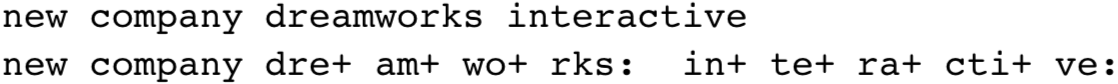
\includegraphics[width=0.45\textwidth]{subword}
	\label{fig:subword}
\end{figure}

Furthermore, the study shows the improvements in performance of language models using subword-level approach instead of character-level. In addition, subword-level language modeling reduces the number of parameters in neural network architecture, which is computed as follows:

\begin{equation}
	\# of parameters = (2 \times V + H) \times H
\end{equation}

where V -- the size of vocabulary, and H -- the size of hidden layer.

Thus, the subword-level language modeling is worth considering for usage in language modeling tasks due to its combination of advantages of both word-level and character-level approaches.

\subsection{Reinforcement Learning}

Reinforcement learning is an area of deep learning with specific agent and environment where agent is rewarded according to its performance on some task. For instance, B.Zaph and Quoc V. Le in their study \cite{Quoc2017Reinforcement} present a novel reinforcement learning algorithm that searches best neural network architecture for performing language modeling tasks (refer to figure \ref{fig:rl}).

\begin{figure}[h]
	\centering
	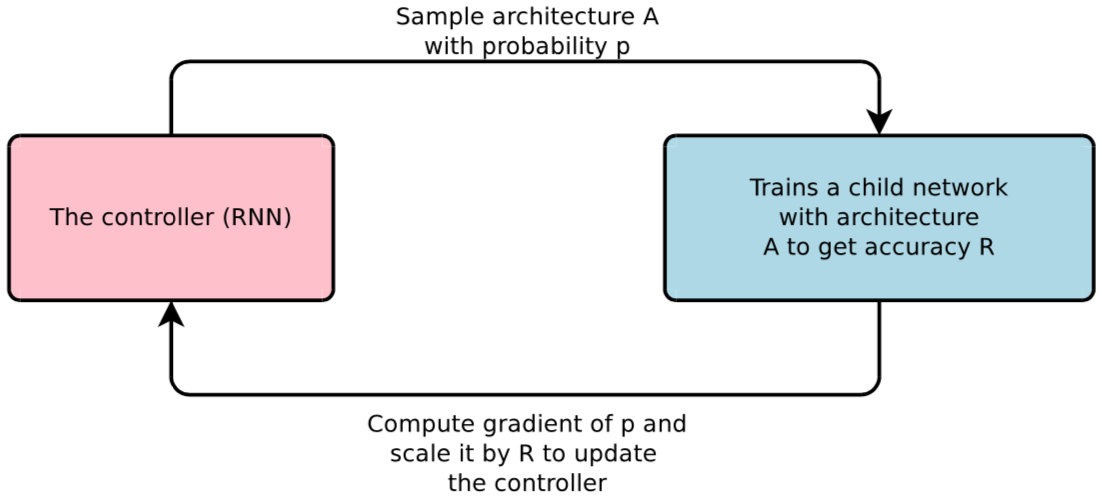
\includegraphics[width=0.5\textwidth]{reinforcement}
	\caption{An overview of Neural Architecture Search from \cite{Quoc2017Reinforcement}}
	\label{fig:rl}
\end{figure}

As it can be seen from figure \ref{fig:rl}, the agent gives reward signal to the controller that tries different neural network architectures based on the accuracy result of the neural network. As a result, the neural network architecture achieves higher accuracy performance further. For better understanding, one may imagine a controller parent recurrent neural network that produce child neural network architecture, and gets rewarded on the performance of the child. It is the same as if the hardware engineer (parent) develops a robot (child), and based on the performance of robot on a given task, the engineer gets rewarded.

The algorithm in \cite{Quoc2017Reinforcement} constructs a tree of architectures which RNN controller then uses. The search space for the controller includes 1) a combination method -- \textit{addition}, \textit{multiplication}, and 2) an activation function -- \textit{identity}, \textit{tanh}, \textit{sigmoid}, \textit{relu}. The authors of \cite{Quoc2017Reinforcement} evaluated the performance of their neural architecture searcher on a well-known dataset for language modeling, Penn Treebank. The table \ref{tab:search} demonstrates the obtained results of \cite{Quoc2017Reinforcement} work.

Hence, reinforcement learning techniques also can support language models with a guidance on how to achieve better accuracy results.

\section{Conclusion and future work}

Language modeling appeared to be a main task in a variety of NLP tasks. Therefore, in the previous century statistical language models were invented to make prediction of next word in the document easier using statistics. However, in the last decades neural language models or also called continous-space language models have started to be used.

Over the past few years, it was clearly seen that continous-space language models outperformed statistical modeling techniques significantly. The ease of feature learning without need in extraction of those features simplified lives of the scientists. The neural approach offers such opportunity to its users.

There was number of studies showing that neural language models outperforms statistical models in terms perplexity and in addition do not require large datasets as backoff models. This leads us to the fact that neural language models are current state-of-the-art techniques in language modeling. Those neural language approaches include feed-forward neural networks, simple recurrent neural networks, improved recurrent neural networks (LSTM) on a word-level and subword-level trained in the standard and non-standard (reinforcement learning) ways.

As we have already observed, there are lots of different neural solutions to language modeling tasks. And as we have seen in \cite{Quoc2017Reinforcement}, combining several techniques results in newer improvements of existing models. So, the study suggests to combine different approaches in the way that will obtain better results in perplexity. For instance, one may combine the subword-level RNN (LSTM) based language model with deep reinforcement learning algorithm.

\bibliographystyle{IEEEtran}
\bibliography{reference}
\printbibliography

\end{document}